\section{Eliminating target variables}

In the previous sections, we included all targets as variables.
In practice, most variables are predetermined, e.g., the target for
concentrations for metabolites is known, it does not need to be optimized.
Optimization algorithms will typically eliminate all such variables in a
presolving step, but we might want to eliminate them manually in order to
reduce matrix sizes.

The procedure is fairly simple: we extract the submatrix corresponding to
targets with known values, multiply it by the value vector, and move it
to the right-hand side~\reffigp{fig:target_elimination}.

\begin{figure}
  \centering
  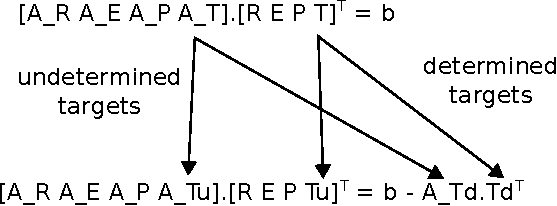
\includegraphics{target_elimination}
  \caption{Procedure to reduce matrix size by eliminating targets
  with predefined values.
  This yield a smaller A matrix and a slightly more complicated b matrix.}
  \label{fig:target_elimination}
\end{figure}
